%% ============================================================================
%% §4.2.2 Operator Engines + Design Rationale  (was: FPGA Frontend)
%% Unified description, both engines + rationale.
%% ============================================================================
\subsubsection{Operator Engines}
\label{sec:hw:frontend:engines}

\paragraph{$1\times1$ Conv engine (14$\times$16 systolic array).}
The $1\times1$ engine is the workhorse of the NPU: $1\times1$ convolution accounts for roughly 92\% of MobileFaceNet's compute. Figure~\ref{fig:engine_1x1} shows its datapath, and Figure~\ref{fig:engine_1x1_dir} shows the spatial-tile sliding direction across the input feature map.

\begin{figure}[H]
  \centering
  \begin{subfigure}{0.62\textwidth}
    \centering
    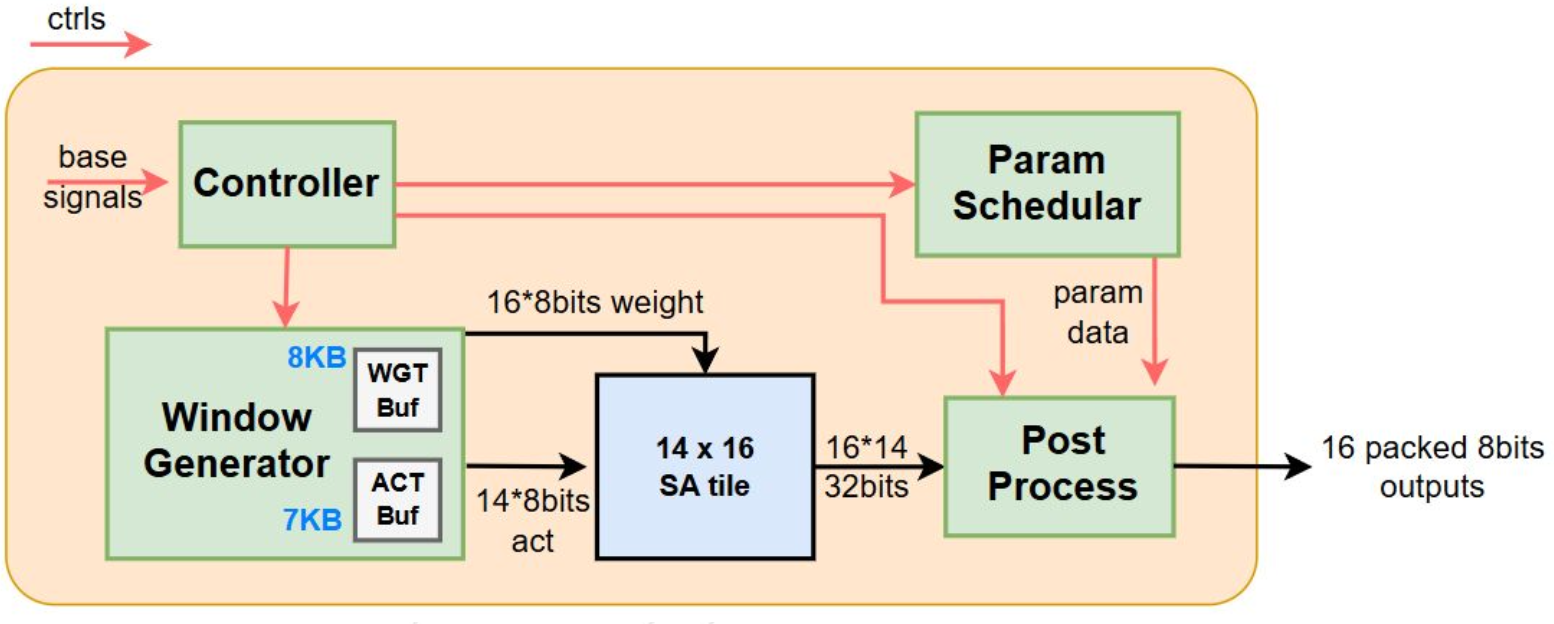
\includegraphics[width=\linewidth]{Fig/peixing/1by1conv.png}
    \caption{$1\times1$ engine block diagram.}
    \label{fig:engine_1x1}
  \end{subfigure}
  \hfill
  \begin{subfigure}{0.32\textwidth}
    \centering
    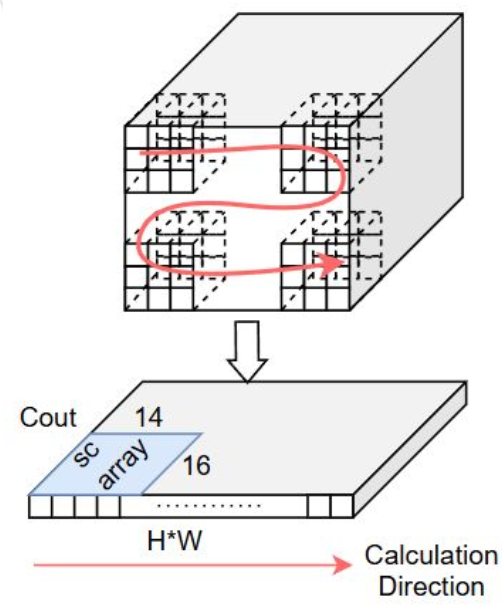
\includegraphics[width=\linewidth]{Fig/peixing/1by1convdirection.png}
    \caption{Sliding direction over $H\times W$.}
    \label{fig:engine_1x1_dir}
  \end{subfigure}
  \caption[$1\times1$ Conv engine and slide direction.]{$1\times1$ Conv engine: 14$\times$16 SA tile fed by a Window Generator with 8\,KB WGT Buf and 7\,KB ACT Buf, outputting 16$\cdot$14 32-bit partial sums per cycle into the Post-Process unit.}
  \label{fig:engine_1x1_pair}
\end{figure}

The Controller drives the Window Generator to load 14 INT8 activations per cycle (one per SA row) and 16 INT8 weights per cycle (one per SA column). The 14$\times$16 = 224-PE tile produces 224 32-bit partial sums per cycle. The Param Scheduler streams bias, requantisation factors, and PReLU $\alpha$ into the Post-Process unit, which packs 16 INT8 outputs into the A/O RAM each cycle.

\paragraph{$3\times3$ Layer engine.}
The $3\times3$ engine handles both standard $3\times3$ convolution and $3\times3$ depthwise convolution. Its datapath is shown in Figure~\ref{fig:engine_3x3}, and the calculation direction (through the input volume) in Figure~\ref{fig:engine_3x3_dir}.

\begin{figure}[H]
  \centering
  \begin{subfigure}{0.62\textwidth}
    \centering
    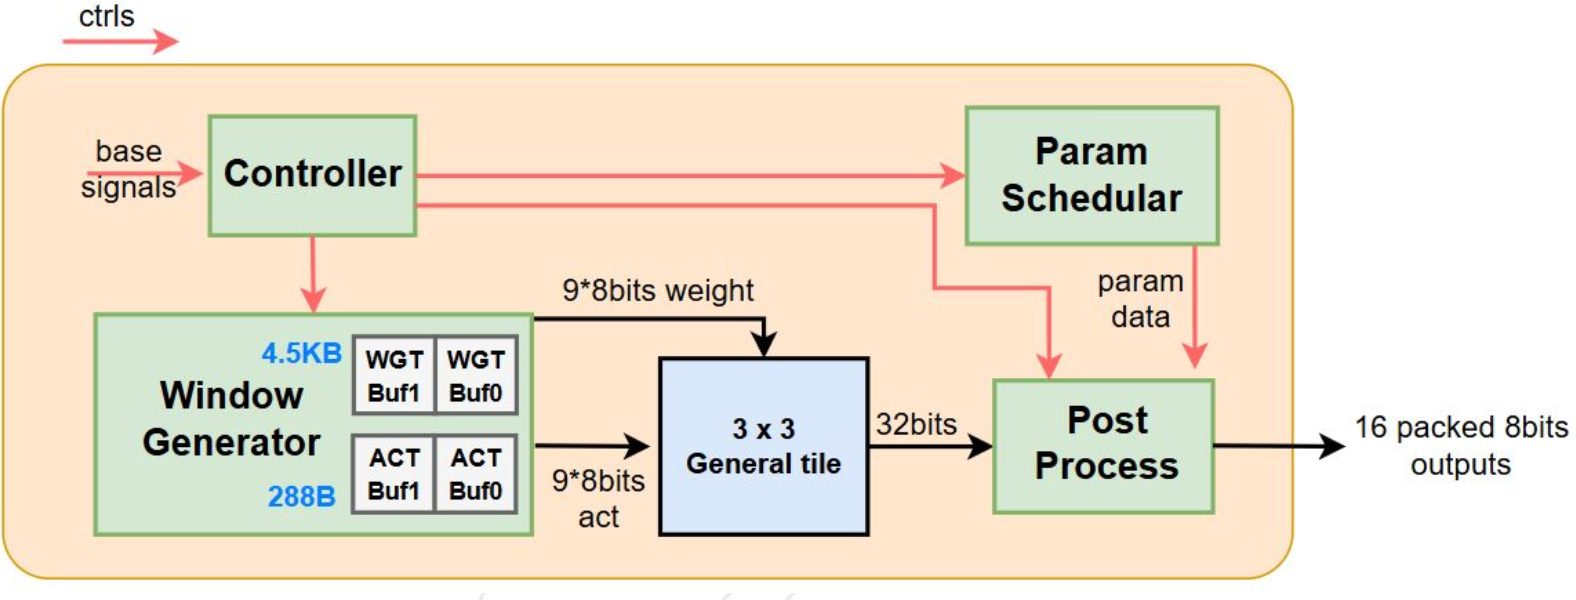
\includegraphics[width=\linewidth]{Fig/peixing/3by3conv.png}
    \caption{$3\times3$ engine block diagram.}
    \label{fig:engine_3x3}
  \end{subfigure}
  \hfill
  \begin{subfigure}{0.32\textwidth}
    \centering
    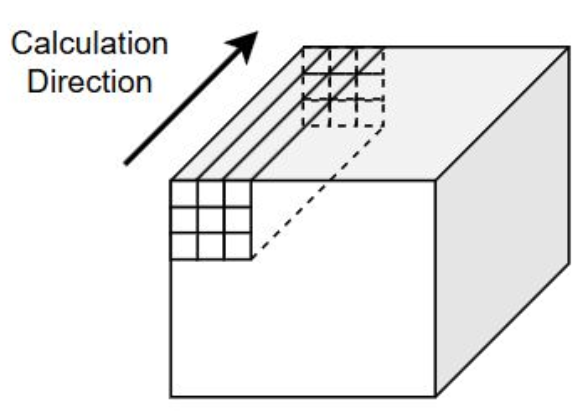
\includegraphics[width=\linewidth]{Fig/peixing/3by3direction.png}
    \caption{Calculation direction.}
    \label{fig:engine_3x3_dir}
  \end{subfigure}
  \caption[$3\times3$ Layer engine and direction.]{$3\times3$ Layer engine: a $3\times3$ general tile fed by a 4.5\,KB WGT buf and a 288\,B ACT buf, with double-buffering (Buf0/Buf1) so the next window is fetched while the current one computes. Outputs 16 packed 8-bit values per cycle.}
  \label{fig:engine_3x3_pair}
\end{figure}

\subsubsection{Design Rationale}
\label{sec:hw:frontend:rationale}

\paragraph{Why a systolic array.}
$1\times1$ convolution dominates the network's compute budget (around 92\%), so the $1\times1$ engine drives most of the area and energy budget. A systolic-array organisation amortises the memory-bandwidth pressure of the dense matrix--vector multiply: the SA tile reuses each fetched weight across 14 spatial positions and each fetched activation across 16 output channels, so per cycle the engine needs only $14+16 = 30$ INT8 reads, against the $14\times16\cdot 2 = 448$ that a fully unrolled MAC array would require. Figure~\ref{fig:why_sa} illustrates the resulting weight-reuse data movement.

\begin{figure}[H]
  \centering
  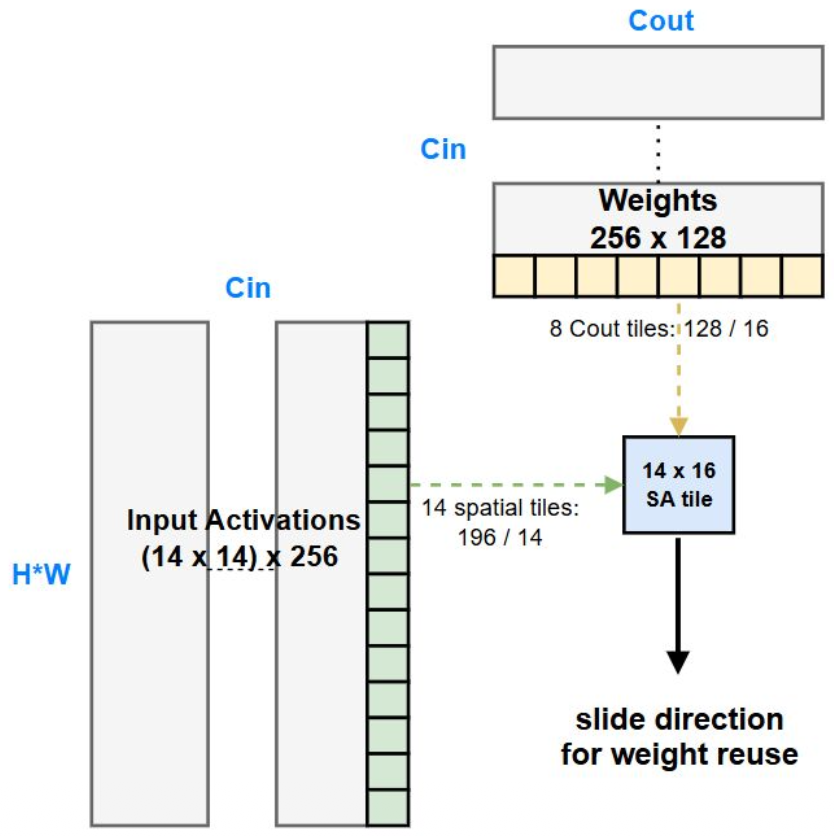
\includegraphics[width=0.85\textwidth]{Fig/peixing/why_systolic_arr.png}
  \caption[Why systolic array.]{Weight-stationary slide direction in the $14\times16$ SA tile: each weight block is held in the array and reused across spatial tiles before the next slide.}
  \label{fig:why_sa}
\end{figure}

\paragraph{Why 14$\times$16.}
MobileFaceNet's recurring dimensions are $H,W \in \{7, 14, 28, 56\}$ and $C_\text{in}, C_\text{out} \in \{64, 128, 256, 512\}$. Setting the SA spatial dimension to 14 lets the engine cover an entire row of a $14\times W$ feature map in one tile (and partially tile rows from $28$ or $56$), and setting the output dimension to 16 divides every $C_\text{out}$ value cleanly. With this choice the layer scheduler never needs to handle awkward residual tiles. A larger SA (e.g.\ 28 or 32 wide) would idle PEs on the smallest $7\times W$ layers; a smaller one would waste reuse on the larger layers.

\paragraph{Quantization scheme.}
Activations carry a non-zero zero-point ($\textit{zp}_a$) and weights are kept symmetric ($\textit{zp}_w = 0$), so the asymmetric-MAC expansion of Eq.~\eqref{eq:quant} collapses to a single $-zp_a \cdot \sum wgt$ correction per output channel, applied off the critical path as part of the bias.

\paragraph{Why not a single oversized array.}
A traditional unified $3\times3$ array was considered for all operators. Two issues made it unattractive: it complicates the outer controller because $1\times1$ and $3\times3$ have very different sliding patterns, and the effective $C_\text{in}$ available to the $3\times3$ array per cycle is only $3\times3\times3 = 27$ for the first layer and $3\times3 = 9$ for depthwise layers, which under-utilises a large array. Splitting the operators across two specialised engines lets each engine match its workload.
